\documentclass[12pt,letter]{article}    

%########################################################################################  
%            						PACKAGES
%######################################################################################## 

\usepackage{amsmath,amsthm,amssymb,bbm,mathrsfs} %math stuff
\usepackage{comment}
\usepackage{caption}
\usepackage{subfig}
\usepackage{float}
\usepackage{authblk}
\usepackage{lscape}
\usepackage{xparse} % FOR CREATING CUSTOM ITEMIZE FUNCTION
\usepackage{lastpage}
\usepackage[linesnumbered,ruled,vlined]{algorithm2e}
\usepackage[round]{natbib}   % omit 'round' option if you prefer square brackets
%\usepackage[numbers,sort]{natbib}   % omit 'round' option if you prefer square brackets
\usepackage{placeins}
\usepackage{epstopdf}
\usepackage{setspace} %Spacing
\usepackage{graphicx,graphics}
\usepackage{booktabs,tabularx}
\usepackage{enumerate}
\usepackage{makecell}
\usepackage{xfrac}
\usepackage{array}
\newcolumntype{L}{>{\centering\arraybackslash}m{3cm}} % used for text wrapping in ctable
\usepackage[nottoc,notlot,notlof]{tocbibind}
\usepackage{tikz}
\usetikzlibrary{trees, shapes.geometric,arrows,shapes.symbols,decorations.pathreplacing,positioning,decorations.markings, fit, matrix}
\usepackage{ctable} % NEED TO LOAD CTABLE AFTER TIKZ FOR SOME REASON
\usepackage[parfill]{parskip} % Activate to begin paragraphs with an empty line rather than an indent
\usepackage[margin=1in]{geometry}

\usepackage[pagebackref=true,bookmarks]{hyperref}
\hypersetup{
    unicode=false,          
    pdftoolbar=true,        
    pdfmenubar=true,        
    pdffitwindow=false,     % window fit to page when opened
    pdfstartview={FitH},    % fits the width of the page to the window
    pdftitle={Protocol},    % title
    pdfauthor={Sahir Rai Bhatnagar},     % author
    pdfsubject={Subject},   % subject of the document
    pdfcreator={Sahir Rai Bhatnagar},   % creator of the document
    pdfproducer={Sahir Rai Bhatnagar}, % producer of the document
    pdfkeywords={}, % list of keywords
    pdfnewwindow=true,      % links in new window
    colorlinks=true,       % false: boxed links; true: colored links
    linkcolor=red,          % color of internal links (change box color with linkbordercolor)
    citecolor=blue,        % color of links to bibliography
    filecolor=black,      % color of file links
    urlcolor=blue           % color of external links
}

 %########################################################################################  
 %            						DEFINE COLORS
 %######################################################################################## 

 \usepackage{color, colortbl, xcolor}
 \definecolor{Gray}{gray}{0.9}
 \definecolor{gray}{RGB}{110,110,110}
 \definecolor{darkgray}{RGB}{100,100,100}
 \definecolor{lightgray}{RGB}{200,200,200}
 \definecolor{turquoise}{RGB}{81,193,188}
 \definecolor{tomato}{RGB}{255,136,136}
 \definecolor{mandarina}{RGB}{229,169,25}
 \definecolor{foreground}{RGB}{81,141,193}
 \definecolor{background}{RGB}{246,244,240}
 \definecolor{highlight}{RGB}{229,169,25}
 \definecolor{lowlight}{RGB}{200,200,200}
 \definecolor{beige}{RGB}{255,255,240}
 \definecolor{pinkish}{RGB}{255,223,247}
 \definecolor{blueish}{RGB}{204,255,255}
 \definecolor{deepink}{RGB}{255,20,147}

 
 %########################################################################################  
 %            						TIKZ SHAPES
 %######################################################################################## 
 

 \tikzstyle{startstop} = [rectangle, rounded corners, minimum width=2cm, minimum height=1cm, draw=black, fill=pinkish,text width=3.5cm]
 \tikzstyle{startstop2} = [rectangle, rounded corners, minimum width=2cm, minimum height=1cm, draw=black, fill=background,text width=3.5cm]
 \tikzstyle{startstop3} = [rectangle, rounded corners, minimum width=3cm, minimum height=1cm, draw=black, fill=beige,text width=3.5cm]
 \tikzstyle{startstop4} = [rectangle, rounded corners, minimum width=3cm, minimum height=1cm, draw=black, fill=blueish,text width=3.5cm]
 \tikzstyle{io} = [trapezium, trapezium left angle=70, trapezium right angle=110, minimum width=2cm, minimum height=1cm, text centered, draw=black, fill=blue!30,text width=1.5cm]
 \tikzstyle{process} = [rectangle, minimum width=1cm, minimum height=1cm, text centered, draw=black, fill=orange!30,text width=2cm]
 \tikzstyle{decision} = [diamond, minimum width=2cm, minimum height=1cm, text centered, draw=black, fill=green!30]
 \tikzstyle{arrow} = [thick,->,>=stealth]
 \tikzstyle{both} = [thick,<->,>=stealth, red]
 \tikzstyle{box} = [rectangle, draw]
 \tikzstyle{line} = [draw, -latex']
 
 \tikzset{myshade/.style={minimum size=.4cm,shading=radial,inner color=white,outer color={#1!90!gray}}}
 \newcommand\mycirc[1][]{\tikz\node[circle,myshade=#1]{};}
 \newcommand\myrect[1][]{\tikz\node[rectangle,myshade=#1]{};}
 \newcommand\mystar[1][]{\tikz\node[star,star points=15,star point height=2pt,myshade=#1]{};}
 \newcommand\mydiamond[1][]{\tikz\node[diamond,myshade=#1]{};}
 \newcommand\myellipse[1][]{\tikz\node[ellipse,myshade=#1]{};}
 \newcommand\mykite[1][]{\tikz\node[kite,myshade=#1]{};}
 \newcommand\mydart[1][]{\tikz\node[dart,myshade=#1]{};}
 \newcommand\mycloud[1][]{\tikz\node[cloud,myshade=#1]{};}
 
 
 \tikzset{
     ncbar angle/.initial=90,
     ncbar/.style={
         to path=(\tikztostart)
         -- ($(\tikztostart)!#1!\pgfkeysvalueof{/tikz/ncbar angle}:(\tikztotarget)$)
         -- ($(\tikztotarget)!($(\tikztostart)!#1!\pgfkeysvalueof{/tikz/ncbar angle}:(\tikztotarget)$)!\pgfkeysvalueof{/tikz/ncbar angle}:(\tikztostart)$)
         -- (\tikztotarget)
     },
     ncbar/.default=0.5cm,
 }
 
 \tikzset{square left brace/.style={ncbar=0.5cm}}
 \tikzset{square right brace/.style={ncbar=-0.5cm}}
 
 \tikzset{round left paren/.style={ncbar=0.4cm,out=110,in=-110}}
 \tikzset{round right paren/.style={ncbar=0.5cm,out=60,in=-60}}

%########################################################################################  
%            						CUSTOM COMMANDS
%######################################################################################## 

\NewDocumentCommand\mylist{>{\SplitList{;}}m}
  {
    \begin{itemize}
      \ProcessList{#1}{ \insertitem }
    \end{itemize}
  }
\newcommand\insertitem[1]{\item #1}

\newcommand{\norm}[1]{\left\Vert #1 \right\Vert}
\newcommand{\code}[1]{\texttt{#1}}
\newcommand{\highcode}[1]{\textcolor{highlight}{\texttt{#1}}}
\newcommand {\bs}{\boldsymbol} 
\newcommand{\bb}{\boldsymbol{\beta}}

\newcommand\independent{\protect\mathpalette{\protect\independenT}{\perp}}
\def\independenT#1#2{\mathrel{\rlap{$#1#2$}\mkern2mu{#1#2}}}
\providecommand{\eeee}[1]{\ensuremath{\times 10^{#1}}}
\setstretch{1} %line spacing

\DeclareMathAlphabet{\mathpzc}{OT1}{pzc}{m}{it}
\newcommand{\tm}[1]{\textrm{{#1}}}
\newcommand{\xf}{\mathcal{X}}
\newcommand{\pfrac}[2]{\left( \frac{#1}{#2}\right)}
\newcommand{\e}{{\mathsf E}}
\newcommand{\bt}{\boldsymbol{\theta}}
\newcommand{\bmu}{\boldsymbol{\mu}}
\newcommand{\bbeta}{\boldsymbol{\beta}}
\newcommand{\bgamma}{\boldsymbol{\gamma}}
\newcommand{\balpha}{\boldsymbol{\alpha}}
\newcommand {\E}{\mathbb{E}} 
\newcommand{\mc}[2]{\multicolumn{#1}{c}{#2}}
\newcommand{\bh}{\hat{\beta}}
\newcommand{\xtx}{\mathbf{X}^T\mathbf{X}}
\newcommand{\xtxinv}{\left(\mathbf{X}^T\mathbf{X}\right)^{-1}}
\newcommand{\mb}[1]{\mathbf{#1}}
\newcommand{\dnorm}[3]{\frac{1}{\sqrt{2\pi #3}} \expp{- \frac{\left( #1-#2\right) ^2}{2 #3}}  }
\newcommand{\dpois}[3]{\frac{\exp\left(-#2\right) #3 }{#1 !}}
\newcommand{\bx}{\mathbf{X}}
\newcommand{\by}{\mathbf{Y}}
\newcommand{\cg}[1]{\textcolor{red}{#1}}
\newcommand{\blanchem}[1]{\textcolor{blue}{#1}}
\newcommand{\mt}[1]{\textcolor{turquoise}{#1}}
\DeclareMathOperator*{\argmin}{arg\,min}


%########################################################################################  
%            						FANCY HEADER STUFF
%######################################################################################## 

\usepackage{fancyhdr}
\cfoot{\thepage}
\lhead[\leftmark]{}
\rhead[]{\leftmark}
\makeatletter
\makeatother
\lfoot{} \cfoot{ } \rfoot{{\small{\em Page \thepage \ of \pageref{LastPage}}}}


%########################################################################################  
%            						SPACING
%######################################################################################## 

%\usepackage{fullpage}
\usepackage[]{titlesec}

\titleclass{\subsubsubsection}{straight}[\subsection]

\newcounter{subsubsubsection}[subsubsection]
\renewcommand\thesubsubsubsection{\thesubsubsection.\arabic{subsubsubsection}}
\renewcommand\theparagraph{\thesubsubsubsection.\arabic{paragraph}} % optional; useful if paragraphs are to be numbered

\titleformat{\subsubsubsection}
  {\normalfont\normalsize\bfseries}{\thesubsubsubsection}{1em}{}
\titlespacing*{\subsubsubsection}
{0pt}{3.25ex plus 1ex minus .2ex}{1.5ex plus .2ex}

\makeatletter
\renewcommand\paragraph{\@startsection{paragraph}{5}{\z@}%
  {3.25ex \@plus1ex \@minus.2ex}%
  {-1em}%
  {\normalfont\normalsize\bfseries}}
\renewcommand\subparagraph{\@startsection{subparagraph}{6}{\parindent}%
  {3.25ex \@plus1ex \@minus .2ex}%
  {-1em}%
  {\normalfont\normalsize\bfseries}}
\def\toclevel@subsubsubsection{4}
\def\toclevel@paragraph{5}
\def\toclevel@paragraph{6}
\def\l@subsubsubsection{\@dottedtocline{4}{7em}{4em}}
\def\l@paragraph{\@dottedtocline{5}{10em}{5em}}
\def\l@subparagraph{\@dottedtocline{6}{14em}{6em}}
\makeatother

\setcounter{secnumdepth}{4}
\setcounter{tocdepth}{4}

%\titlespacing*{\section}{0pt}{-1ex}{-1ex}
%\titlespacing*{\subsection}{0pt}{-1ex}{-1ex}
%\titlespacing*{\subsubsection}{0pt}{-1ex}{-1ex} 

%\renewcommand{\headrulewidth}{0.0pt}
%\renewcommand{\footrulewidth}{0.0pt}

%\setlength{\textheight}{9.00in}
%\setlength{\textwidth}{7.00in}
%\setlength{\topmargin}{-0.5in}
%\setlength{\evensidemargin}{-0.25in}
%\setlength{\oddsidemargin}{-0.25in}
%\renewcommand{\baselinestretch}{1.0}
\title{Variable Selection In Additive Gene Environment Interactions with the Group Lasso}
\author{Sahir Bhatnagar and Yi Yang}


%########################################################################################  
%            						START OF DOCUMENT
%########################################################################################  


\begin{document}


\newpage
\pagestyle{fancy}

\maketitle
\section{Introduction}



We consider a regression model for an outcome variable $\mathbf{Y}=(Y_1, \ldots, Y_n)$ where $n$ is the number of subjects. Let $E=(E_1, \ldots, E_n)$ be a binary or continuous environment vector and \mbox{$\bx = (X_{1}, \ldots, X_{n})^T$} be the $n \times p$ matrix of high-dimensional data where $X_i = (X_{i1}, \ldots,X_{ij}, \ldots,  X_{ip}) \in [0,1]^p$. Consider the regression model with main effects and their interactions with $E$:

\begin{equation}  
Y_i = \beta^*_0 + \sum_{j=1}^p \beta^*_j X_{ij} + \beta^*_E E_i + \sum_{j=1}^p \alpha^*_j E_i X_j + \varepsilon_i, \qquad i=1, \ldots, n \label{eq:linpred1.1},
\end{equation}

were $\beta^*_0,\beta^*_j,\beta^*_E,\alpha^*_j$ are the true unknown model parameters for $j=1, \ldots, p$. This can be extended to the more general additive model:

\begin{equation}  
Y_i = \beta^*_0 + \sum_{j=1}^p f^*_j (X_{ij}) + f_E^*(E_i) + \sum_{j=1}^p f^*_{jE} (X_{ij},E_i) + \varepsilon_i \qquad i=1, \ldots, n \label{eq:linpred1.2}
\end{equation}

As in~\citep{radchenko2010variable}, we can express~\eqref{eq:linpred1.2} as 
\begin{equation}
\mb{Y} =  \sum_{j=1}^p \mb{f}^*_j + \mb{f}_E^*(E_i) + \sum_{j=1}^p \mb{f}^*_{jE} + \varepsilon_i 
\end{equation}
where $\mb{f}^*_j = \left(f_j^*(X_{1j}), \ldots, f_j^*(X_{nj})\right)^T$, $\mb{f}^*_{jE} = \left(f_{jE}^*(X_{1j},X_{1E}), \ldots, f_j^*(X_{nj}, X_{nE})\right)^T$














\newpage
%\bibliographystyle{plainnat}
%\addcontentsline{toc}{chapter}{References}
\bibliographystyle{unsrtnat}
\bibliography{/home/sahir/Dropbox/PhD/Protocol/GEbib}


\end{document}


\subsection{Main Idea}
This manuscript addresses more traditional \textit{statistical} interaction models of the form 

\begin{equation}
Y = X\beta_X + E \beta_E + X E \beta_{XE} + \varepsilon
\end{equation}

We propose to first filter out the noise variables (main effects only) using a method from the \textit{variable screening} literature, and then subsequently fit a penalized model, on the filtered set of variables, that enforces the strong heredity property, i.e., interaction terms can only be selected by the procedure if the main effects have been selected. 


\subsection{Introduction}

We consider a regression model for an outcome variable $Y=(y_1, \ldots, y_n)$ which follows an exponential family. Let $E=(e_1, \ldots, e_n)$ be the binary environment vector and $\bx = (X_{1}, \ldots, X_{p})$ be the matrix of high-dimensional data. Consider the regression model with main effects and their interactions with $E$:
\begin{align}
g(\bmu)  = & \beta_0  + \underbrace{\beta_1 X_{1} + \cdots + \beta_p X_p + \beta_{E} E}_{\tm{main effects}} + \underbrace{\alpha_{1E} (X_1 E) + \cdots + \alpha_{pE} (X_p E)}_{\tm{interactions}} \label{eq:linpred1}
\end{align}
where $g(\cdot)$ is a known link function and $\bmu = \e\left[Y|\bx, E, \bbeta,\balpha\right]$. Our goal is to estimate the parameters \mbox{$\bbeta = \left(\beta_1, \beta_2, \ldots, \beta_p, \beta_E\right) \in \mathbb{R}^{p+1}$} and $\boldsymbol{\alpha} = \left(\alpha_{1E}, \ldots, \alpha_{pE}\right) \in \mathbb{R}^p$ and to improve prediction of $Y$. 

\subsection{Methods} \label{sec:varselect}

\subsubsection{Variable Screening}

Consider a binary response variable $Y=0,1$. A variable $X$ is independent of $Y$ \textit{iff} the conditional distributions of $X$ given $Y=0$ or $Y=1$ are identical. \citep{mai2012kolmogorov} proposed using the Kolmogorov-Smirnov (KS) test statistic
\begin{equation}
\hat{K}_j = \sup_x \lvert \hat{F}_j(x|Y=1) - \hat{F}_j(x|Y=0)  \rvert   \label{eq:ks}
\end{equation}
to measure the dependence between $X_j$ and $Y$, where $\hat{F}_j$ is the empirical CDF of $X_j$. 

\citep{mai2015fused} then extended their method to a continuous response by essentially categorizing the response variable so that Eq.~\eqref{eq:ks} can be applied. They called this the Fused Kolmogorov filter.

\begin{figure}[H]
\centering
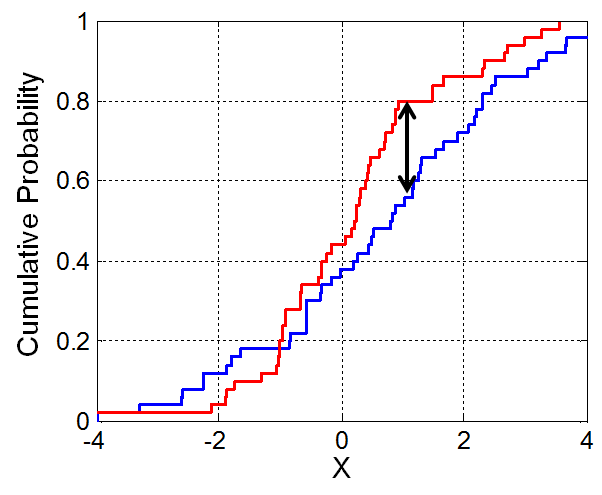
\includegraphics[scale=0.75]{./ks}
\caption{Depiction of KS statistic}
\label{fig:ks}
\end{figure}


\subsubsection{Strong Heredity Model}

We are interested in imposing the strong heredity principle~\citep{chipman1996bayesian}: 
\begin{equation}
\hat{\alpha}_{jE} \neq 0 \qquad \Rightarrow \qquad \hat{\beta}_j \neq 0 \qquad \tm{and} \qquad \hat{\beta}_E \neq 0   \label{eq:heredity}
\end{equation}
In words, the interaction term will only have a non-zero estimate if its corresponding main effects are estimated to be non-zero. One benefit brought by hierarchy is that the number of measured variables can be reduced, referred to as practical sparsity~\citep{she2014group,bien2013lasso}. For example, a model involving $X_1, E, X_1 \cdot E$ is more parsimonious than a model involving $X_1, E, X_2 \cdot E$, because in the first model a researcher would only have to measure two variables compared to three in the second model. In order to address these issues, we propose to extend the model of Choi \textit{et al.}~\citep{choi2010variable} to simultaneously perform variable selection, estimation and impose the strong heredity principle in the context of high dimensional interactions with the environment (HD$\times E$). To do so, we follow Choi and reparametrize the coefficients for the interaction terms as $\alpha_{jE} = \gamma_{jE} \beta_j \beta_E$. Plugging this into~\eqref{eq:linpred1}:
\begin{align}
g(\bmu)  = & \beta_0  + \beta_1 \widetilde{X}_{1} + \cdots + \beta_q \widetilde{X}_q + \beta_{E} E + \gamma_{1E}\beta_1 \beta_E (\widetilde{X}_1 E) + \cdots + \gamma_{qE}\beta_q \beta_E (\widetilde{X}_q E)    \label{eq:linpred2}
\end{align}
where $\widetilde{\bx} = (\widetilde{X}_1, \ldots, \widetilde{X}_q)$ are the cluster representatives derived in phase 2 and $q <p$. This reparametrization directly enforces the strong heredity principle (Eq.~\eqref{eq:heredity}), i.e., if either main effect estimates are 0, then $\hat{\alpha}_{jE}$ will be zero and a non-zero interaction coefficient implies non-zero $\hat{\beta}_j$ and $\hat{\beta}_E$. To perform variable selection in this new parametrization, we follow Choi \textit{et al.}~\citep{choi2010variable} and penalize $\bs{\gamma} = \left(\gamma_{1E}, \ldots, \gamma_{pE}\right)$, leading to the following penalized least squares criterion:
\begin{equation}
\argmin_{\beta_0, \bbeta, \bs{\gamma} }  \frac{1}{2} \norm{Y - g(\bmu)}^2 + \lambda_\beta \left(w_1 \beta_1 + \cdots + w_q \beta_q + w_E \beta_E   \right) + \lambda_\gamma  \left( w_{1E} \gamma_{1E} + \cdots + w_{qE}\gamma_{qE}         \right) \label{eq:lassolikelihood2}
\end{equation} 
where $g(\bmu)$ is from~\eqref{eq:linpred2}, $\lambda_\beta$ and $\lambda_\gamma$ are tuning parameters and $\mb{w} = \left(w_{1}, \ldots, w_q, w_{1E}, \ldots, w_{qE}\right)$ are prespecified adaptive weights. The $\lambda_\beta$ tuning parameter controls the amount of shrinkage applied to the main effects, while $\lambda_\gamma$ controls the interaction estimates and allows for the possibility of excluding the interaction term from the model even if the corresponding main effects are non-zero. The adaptive weights serve as a way of allowing parameters to be penalized differently. Furthermore, adaptive weighting~\citep{zou2006adaptive} has been shown to construct oracle procedures~\citep{fan2001variable}, i.e., asymptotically, it performs as well as if the true model were given in advance. The oracle property is achieved when the weights are a function of any root-$n$ consistent estimator of the true parameters e.g. maximum likelihood (MLE) or ridge regression estimates. It can be shown that the procedure in~\eqref{eq:lassolikelihood2} asymptotically possesses the oracle property~\citep{choi2010variable}, even when the number of parameters tends to $\infty$ as the sample size increases, if the weights are chosen such that
\begin{equation}
w_j = \left | \frac{1}{\hat{\beta}_j} \right|, \quad w_{jE} = \left | \frac{\hat{\beta}_j \hat{\beta}_E}{\hat{\alpha}_{jE}} \right| \quad \tm{ for }j=1, \ldots, q   \label{eq:weights}
\end{equation}
where $\hat{\beta}_j$ and $\hat{\alpha}_{j}$ are the MLEs, \textit{using the transformed variables}, from~\eqref{eq:linpred1} or the ridge regression estimates when $q > n$. The rationale behind the data-dependent $\hat{\bs{w}}$ is that as the sample size grows, the weights for the truly zero predictors go to $\infty$ (which translates to a large penalty), whereas the weights for the truly non-zero predictors converge to a finite constant~\citep{zou2006adaptive}. 

There have been several more recent proposals for modeling interactions with the strong heredity constraint in the variable selection via penalization literature including Composite Absolute Penalties (CAP)~\citep{zhao2009composite}, Variable selection using Adaptive Nonlinear Interaction Structures in High dimensions (VANISH)~\citep{radchenko2010variable}, Strong Hierarchical Lasso (hierNet)~\citep{bien2013lasso}, Group-Lasso Interaction Network (glinternet)~\citep{lim2014learning}, Group Regularized Estimation under Structural Hierarchy (GRESH)~\citep{she2014group} and a Framework for Modeling Interactions with a Convex Penalty (FAMILY)~\citep{haris2014convex}. While each method has their own merit, including that they are all convex optimization problems, they all contain complex penalty functions which are hard to interpret and lead to computationally expensive fitting algorithms. On the other hand, the objective function in~\eqref{eq:lassolikelihood2} can be solved using an iterative approach (by first fixing $\bbeta$ and then $\balpha$) which simplifies to a LASSO type problem; one that has been extensively studied, is well understood and can be solved efficiently using existing software (e.g. \texttt{glmnet}~\citep{friedman2010regularization}). A limitation of this approach is that the optimization problem is non-convex, arising from the reparametrization of $\balpha$ as a product of optimization variables $(\bbeta, \bs{\gamma})$, and hence convergence to the global minimum is not guaranteed~\citep{choi2010variable}. 


\subsection{Simulation Study}


\subsection{Real-Data Example}


\subsection{Novelty and Contributions}

The fused Kolmogorov filter with the strong heredity model has not been previously investigated. 

To our knowledge, strong hierarchies have never previously been used in HD interaction analysis in genomics or brain imaging studies. Furthermore, the specific choices of weights proposed here, i.e., based on the transformed variables from phase 2, have not been previously used. Choi \textit{et al.}~\citep{choi2010variable} estimated their weights simultaneously, but this would not be feasible in HD data. The adaptation to interactions with one key $E$ variable is specific to our situation.

References~\cite{radchenko2010variable,zhao2009composite,she2014group,choi2010variable} (which includes the one that our proposal is based on) failed to provide any code or software for their method. Not only does this prevent applied researchers from using these advanced techniques, it also hinders statisticians from comparing the performance of their newly developed method against existing approaches. Indeed, a survey of the citations of these papers reveals that they are seldom used in practice or as a comparison method in theoretical papers, and only cited in literature review paragraphs. Three approaches that have provided \texttt{R} packages (\texttt{hierNet}~\citep{bien2013lasso}, \texttt{glinternet}~\citep{lim2014learning} and \texttt{FAMILY}~\citep{haris2014convex}) are only suited for all pairwise interactions of the design matrix (the theory in \texttt{FAMILY} does not impose such a restriction but the software returns an error when we input a 1 column environment variable) and are not designed for the HD$\times E$ interactions that are the focus of this thesis. Therefore, a novel aspect of this thesis will be the development of a procedure for $\tm{HD}\times E$ interactions which simultaneously performs variable selection and estimation, follows the strong heredity principle and is an oracle procedure, as well as its implementation into a computationally fast open source \texttt{R} package.


